\documentclass{beamer}
\usepackage[brazil]{babel}
\usepackage{amsmath}
\usepackage{graphicx}
\usepackage{fancybox}
\usetheme{Copenhagen}
%Information to be included in the title page:
\title{Grupos Livres e o Lema do Ping-Pong}
\author{Eric Vaz de Souza Santos}
\institute{Universidade Federal de Sergipe}
\date[2025]
{XVI Escola de Verão em Matemática da UFS}


\expandafter\def\expandafter\insertshorttitle\expandafter{%
  \insertshorttitle\hfill%
  \insertframenumber\,/\,\inserttotalframenumber}
\begin{document}

\frame{\titlepage}

\begin{frame}
\frametitle{Grupos Livres}
O grupo livre sobre um conjunto $S$ é o grupo de palavras reduzidas em $S$ com a operação de concatenação. Denota-se $F_S$
\begin{example}
    Seja $S = \{a,b,c\}$. Então $x = b^{-1}ac^2a^{-2}$ é um elemento de $F_S$.

    A palavra $a b b^{-1} c^2 c$ deve ser reduzida para $y = ac^3$. Note que

    \[xy = (b^{-1}ac^2a^{-2})(ac^3) = b^{-1}ac^2a^{-1}c^3\]
\end{example}

\pause
\begin{example}
    O grupo dos inteiros $\mathbb{Z}$ isomorfo ao grupo livre com apenas um gerador. Este é o único grupo livre abeliano.
\end{example}
\end{frame}

\begin{frame}
    \frametitle{Ações de Grupos}

    \begin{definition}
    Se $G$ é um grupo, uma \textit{ação} de $G$ em $X$ é um homomorfismo $\varphi: G \to \text{Bij}(X)$.
    Denotamos o elemento $\varphi(g)(x)$ por $g \cdot x$.
    \end{definition}

    \pause
    \begin{example}
        O grupo $SO(3, \mathbb{R})$ de todas as matrizes reais $3\times 3$ ortogonais de determinante $1$ age na esfera $S^2\subset\mathbb{R}^3$ por rotações.
    \end{example}

    \pause
    \begin{example}
        O grupo $SO(2,1,\mathbb{R})$ de todas as matrizes de determinante $1$ que preservam a forma quadrática $x^2 + y^2 - z^2$ age no hiperboloide de uma folha $\{x^2+y^2-z^2 = 1\}\subset\mathbb{R}^3$ por transformações de Lorentz.
    \end{example}
\end{frame}

\begin{frame}
    \frametitle{O Lema do Ping-Pong}

    \begin{lemma}
        Seja $G = \langle a, b\rangle$ um grupo com dois geradores que age em um conjunto $X$. Suponha que
        \begin{itemize}
            \item Existem subconjuntos disjuntos $X_a, X_b\subset X$.
            \item $a^k(X_b)\subset X_a$ e $b^k(X_a)\subset X_b$ para qualquer $k\in\mathbb{Z}\setminus\{0\}$.
        \end{itemize}
        Então $G = F_{\{a,b\}}$.
    \end{lemma}
\end{frame}

\begin{frame}
    \begin{proof}
        Basta mostrar que nenhuma palavra não-trivial em $a$ e $b$ é igual à identidade. Seja
        \[w = a^{m_1}b^{n_1}a^{m_2}b^{n_2}\cdots a^{m_k}b^{n_k}\]
        uma palavra reduzida. Conjugando por $a^{m}$, $m\neq -m_1$ não nulo, obtemo uma palavra que começa e termina com $a$:
        \[a^{m} w a^{-m} = a^{m_1 + m}b^{n_1}a^{m_2}b^{n_2}\cdots a^{m_k}b^{n_k}a^{-m}.\]
        Aplicando em $X_b$:
        \begin{align*}
            (a^{m} w a^{-m})(X_b) &= a^{m_1 + m}b^{n_1}a^{m_2}b^{n_2}\cdots a^{m_k}b^{n_k}a^{-m}(X_b)\\
            &\subset\ldots\subset  a^{m_1 + m}b^{n_1}(X_a) \subset a^{m_1 + m}(X_b) \subset X_a.
        \end{align*}
    \end{proof}
\end{frame}

\begin{frame}
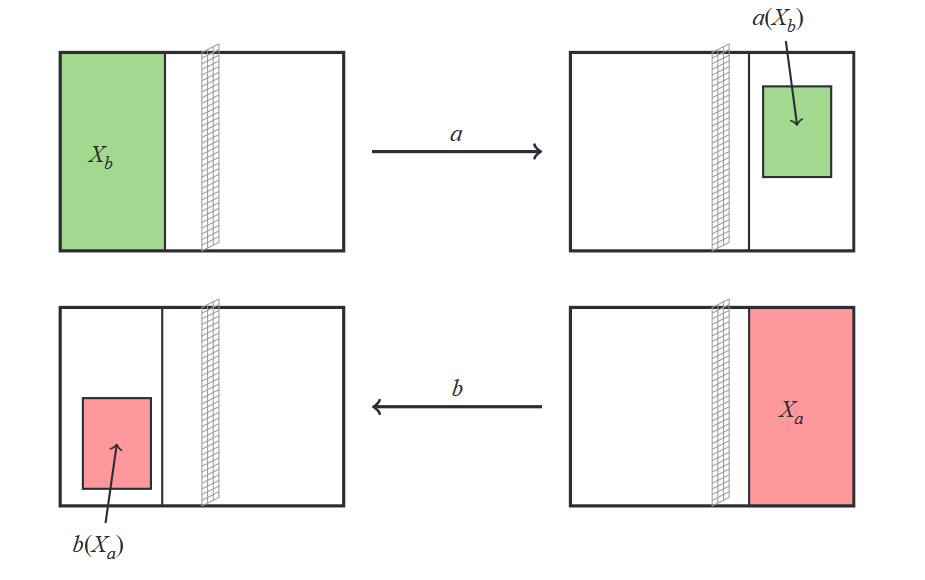
\includegraphics[width=\textwidth]{pong.PNG}
\end{frame}

\begin{frame}
    \frametitle{A esfera de Riemann}
    \begin{definition}
        A esfera de Riemann $\mathbb{CP}^1 = \mathbb{C}\cup\{\infty\}$ é o espaço obtido como o quociente
        \[\frac{\mathbb{C}^2\setminus\{(0,0)\}}{\sim},\]
        onde $(z_1,z_2)\sim (\lambda z_1, \lambda z_2)$ para todo $\lambda\in\mathbb{C}\setminus\{0\}$.
    \end{definition}
    \pause
    \begin{exampleblock}{}
        Um número complexo $z\in\mathbb{C}$ é identificado com a classe de equivalencia $[z,1]$. O ponto $\infty$ é a classe de equivalência $[1,0]$.
    \end{exampleblock}
\end{frame}

\begin{frame}
    \frametitle{Transformações de Möbius}

    \begin{exampleblock}{}
        Uma matriz invertível $\begin{pmatrix}
            a & b\\
            c & d
        \end{pmatrix}$ induz uma função $f : \mathbb{CP}^1\to\mathbb{CP}^1$.
        Estas funções são chamadas de transformações de Möbius.
    \end{exampleblock}
    \pause
    \begin{exampleblock}{}
    Podemos escrever
        \[f(z) = \frac{az+b}{cz+d};\]
        \[f(\infty) = \frac{a}{c};\quad f\left(\frac{-d}{c}\right) = \infty.\]
    \end{exampleblock}
\end{frame}
\begin{frame}
    \frametitle{Pontos fixos de transformações de Möbius}
    \begin{exampleblock}{}
        Note que $f(z) = z$ se, e somente se, $[z:1]$ é um autovetor da matriz correspondente $\begin{pmatrix}
            a & b\\
            c & d
        \end{pmatrix}$.
    \end{exampleblock}
    \pause
    \begin{example}
        \begin{itemize}
            \item A transformação $f(z) = 9z$ tem dois pontos fixos: $0$ e $\infty$.
            \item A transformação $f(z) = \frac{5z + 4}{4z + 5}$ tem dois pontos fixos: $1$ e $-1$.
        \end{itemize}
    \end{example}

    \begin{exampleblock}
        Quando $f$ tem dois pontos fixos distintos, dizemos que $f$ é hiperbólica. Neste caso, 
    \end{exampleblock}
    

\end{frame}

\end{document}